%&spell
\section[Differential branching fraction of the decay \btokpipimumu]
{Differential branching fraction of the decay \tmath{\btokpipimumu}}
%Binning scheme in
      %decays~\cite{LHCb-PAPER-2013-017,LHCb-PAPER-2013-037,LHCb-PAPER-2013-019}.

Given the statistics available for this channel, the differential branching fraction,
$\dBF(\btokpipimumu)/\dqsq$ was calculated in five bins of \qsq with respect to the normalization
channel \btopsitwosk.
This normalization channel is chosen because it has the same final state particle if
\psitwostojpsipipi and \jpsitomumu.
This has a total branching fraction of
$\BF_\mathrm{tot}\big(\btopsitwosk\big) = (1.264 \pm 0.0052)\e{-5}$~\cite{PDG2012},
which has a relative uncertainty of $4\pc$, the alternative normalization channel is
\btojpsikpipi but this has a relative uncertainty of $16\pc$.
%This was chosen for the normalization channel over the decay \btojpsikpipi because it has a
%relative uncertainty of $4\,\%$ rather than $16\,\%$ for $\BF(\btojpsikpipi) = (8.1\pm1.3)\e{-4}$.

The differential branching fraction for a bin of width $\Delta\qsq$ is calculated
%\begin{equation}
  %\frac{d}{\dqsq}\BF\left(\btokpipimumu\right)
  %=
  %\frac{\num{sig}}{\num{norm}} \cdot
  %\frac{\eff{norm}}{\eff{sig}} \cdot
  %\frac{\BF_\mathrm{tot}\left(\btopsitwosk\right)}{\Delta\qsq}
%\end{equation}
\begin{multline}
  \frac{d}{\dqsq}\BF\big(\btokpipimumu\big)=
  \\
  \frac{1}{\Delta\qsq} \cdot
  \frac{N\big(\btokpipimumu\big)}{N\big(\btopsitwosk\big)} \cdot
  \frac{\varepsilon\big(\btopsitwosk\big)}{\varepsilon\big(\btokpipimumu\big)} \cdot
  \BF_\mathrm{tot}\big(\btopsitwosk\big)
  \label{eq:kpipi:diffbf}
\end{multline}
where $N$ and $\varepsilon$ denote yields and efficiencies, respectively.
%\begin{equation*}
%\end{equation*}
%\num{sig} is the yield of the signal decay \btokpipimumu in the given \qsq bin and \num{norm}
%is the yield of the normalization channel.
%Total deficiencies for reconstruction and selection are denoted by \eff{sig} and \eff{norm} for the
%signal and normalization channels respectively.


The yield  of the normalization channel is extracted from an unbinned extended maximum likelihood
fit to the invariant mass distribution of \btopsitwosk candidates.
%The function used to fit the data constitutes a signal and background component.
The signal shape is modelled using the sum of two Gaussian functions, each having a power-law
tail at low-mass, where the tail parameters are shared between both Gaussians.
Two Gaussian functions are due to different resolution effects, the wider one is due to events
where tracks have been through the \ot or undergone multiple scattering.
Background is modelled using the sum of an exponential to model combinatorial background, and a
Gaussian at low mass to model partially reconstructed candidates.
The control channel \btojpsikpipi is fit to the same model.
These fits are shown in \Fig{fig:kpipi:norm} and they yield
$N\big(\btopsitwosk\big)=5128\pm67$ and $N\big(\btojpsikpipi\big)=59\,335\pm343$.

\begin{figure}
  \begin{center}
    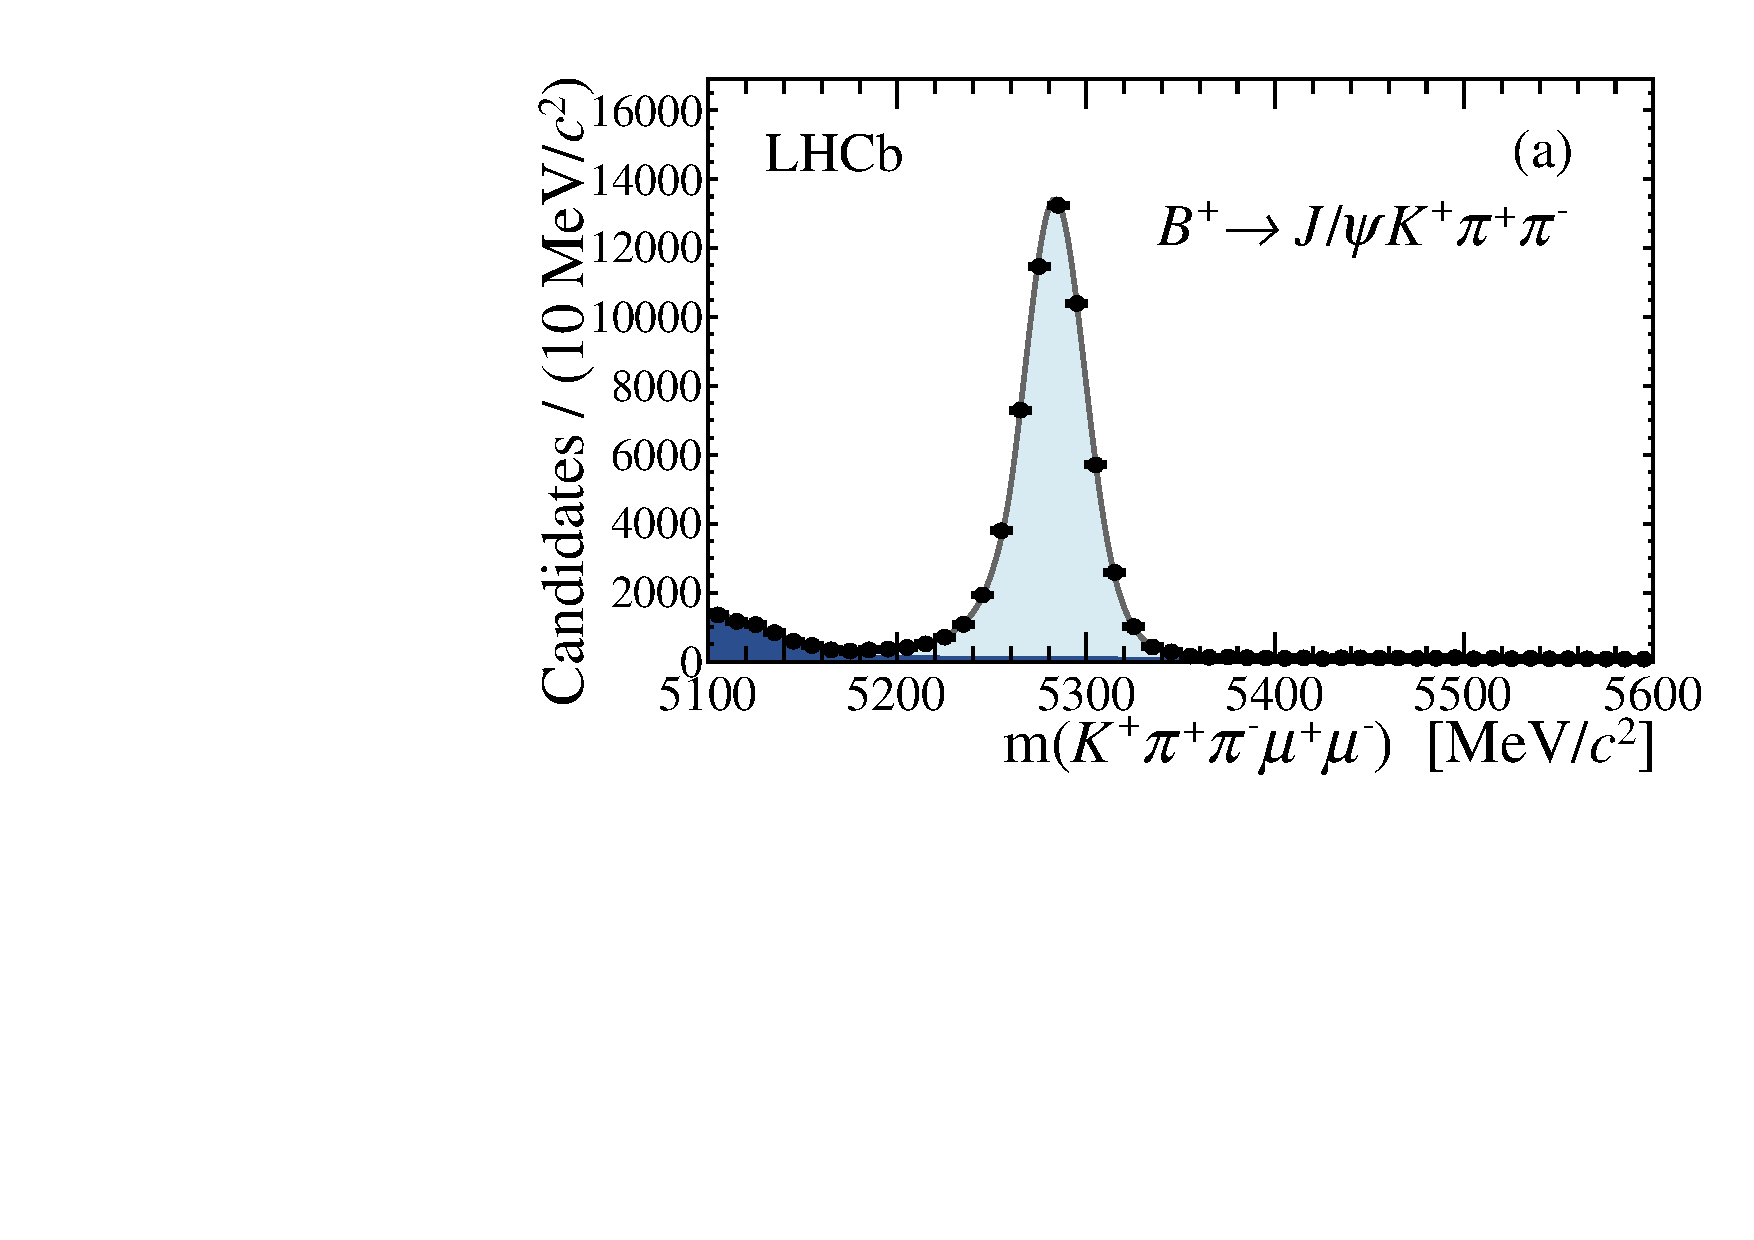
\includegraphics[width=0.48\textwidth]{b2kpipijpsi}
    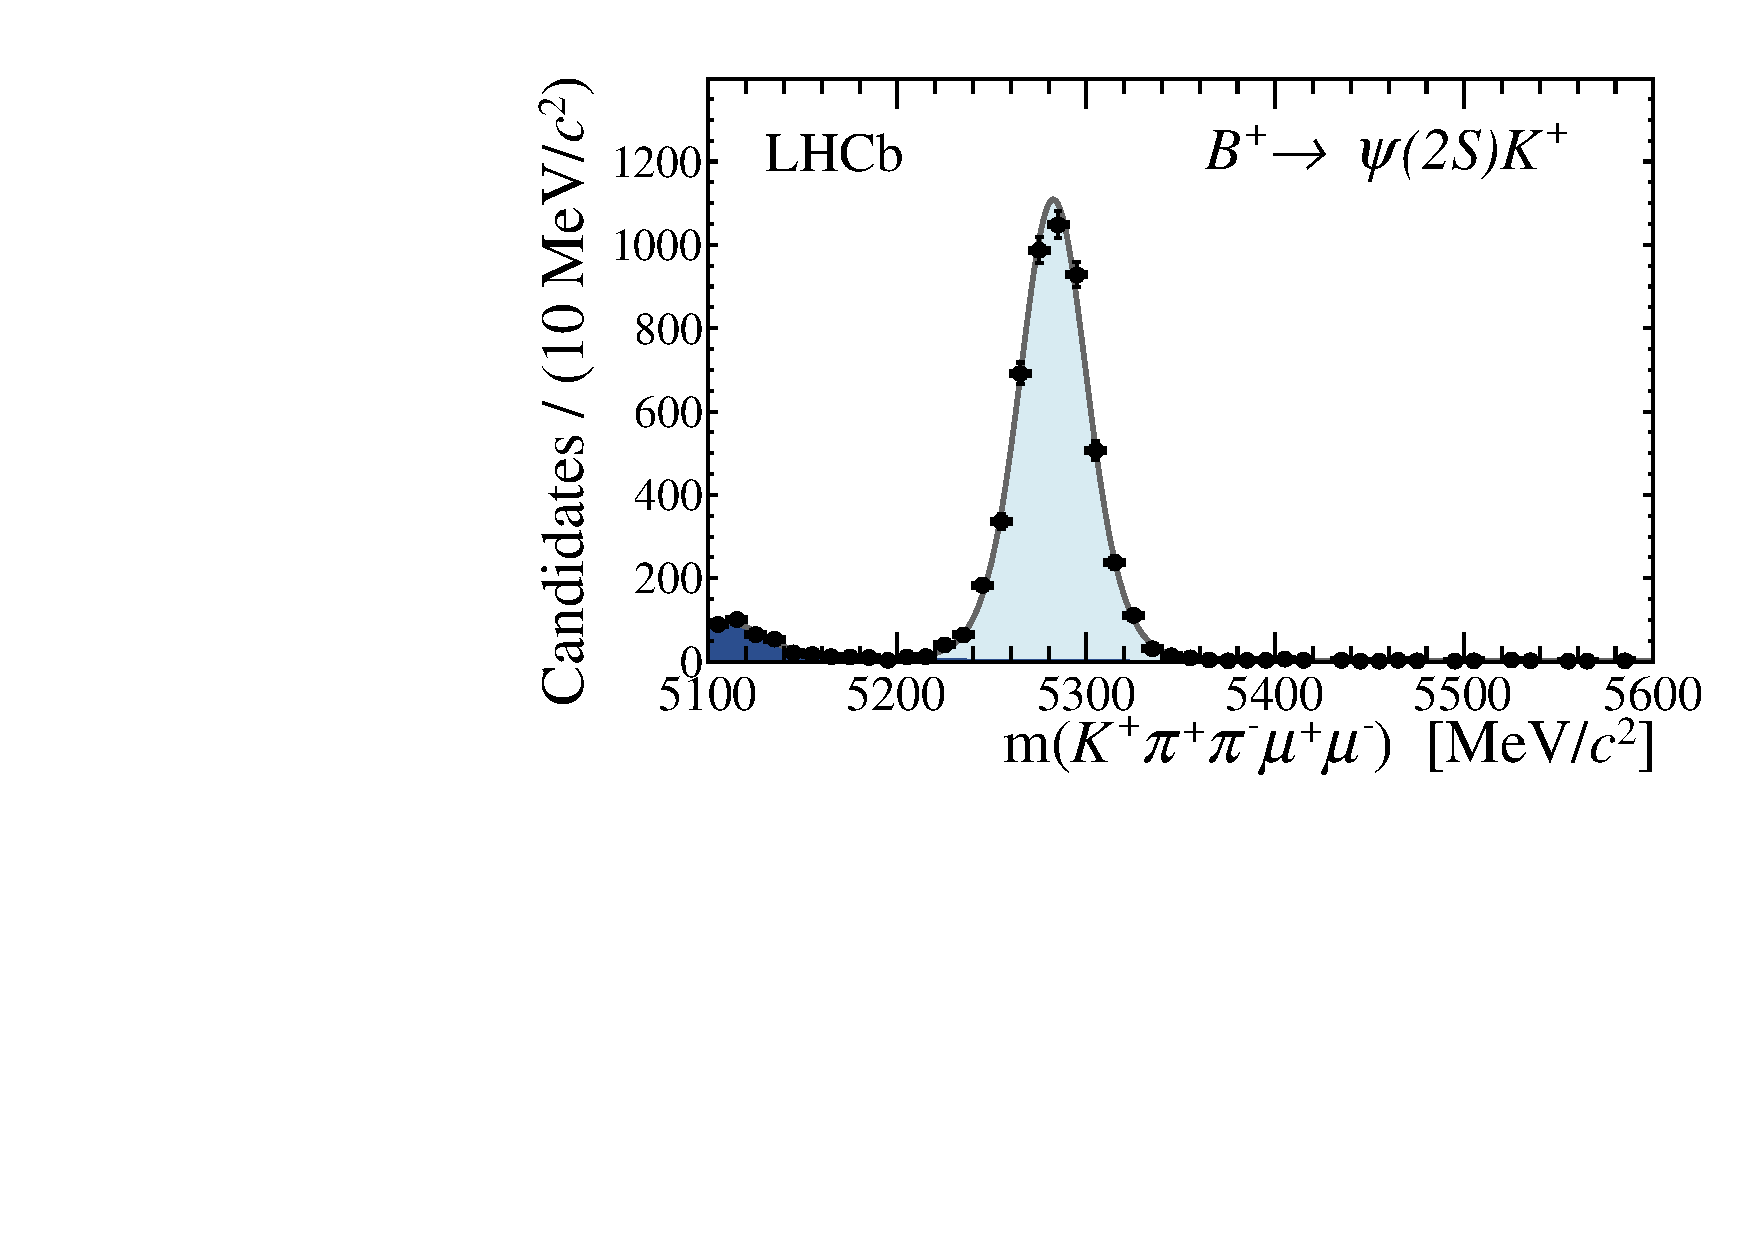
\includegraphics[width=0.48\textwidth]{b2psi2sk}
    \caption[Fits to \btojpsikpipi and \btopsitwosk candidates]
    {
      Distributions of the invariant mass of the
      (left) cross-check channel \btojpsikpipi and
      (right) normalization mode \btopsitwosk.
      Projections from the fit are overlayed, where the light blue is the yield of the indicated
      decay, and the dark blue is the background component.
    }
    \label{fig:kpipi:norm}
  \end{center}
\end{figure}


Yields of the signal decay in regions of \qsq were extracted from fits using a distribution that
was fixed to as large an extent as possible.
The lower limit of the fit was taken to be $5150\mev$, because partially reconstructed background
becomes significant below that.
The combinatorial background shape is an exponential distribution, where the exponent and yield was
allowed to float in the fit.
In \qsq regions where charmonium vetoes are effective, the background distribution must account for
the areas in which charmonium vetoes are extended, this is done by incorporating discrete steps in
the combinatorial background; the size of which are determined from data.
%The signal function was also the sum of Gaussians with power law tails, where the parameters are
%all fixed to the values from the fit to the cross-check channel.
A fit from the crosscheck channel fixes the signal model used in the lower statistics signal
channel.
Figure~\ref{fig:kpipi:q2fits} shows the invariant mass distribution for all signal
candidates for the whole \qsq region and for each bin.
The total signal yield is measured to be $N(\btokpipimumu)=367\,^{+24}_{-23}$.

\begin{figure}
  \begin{center}
    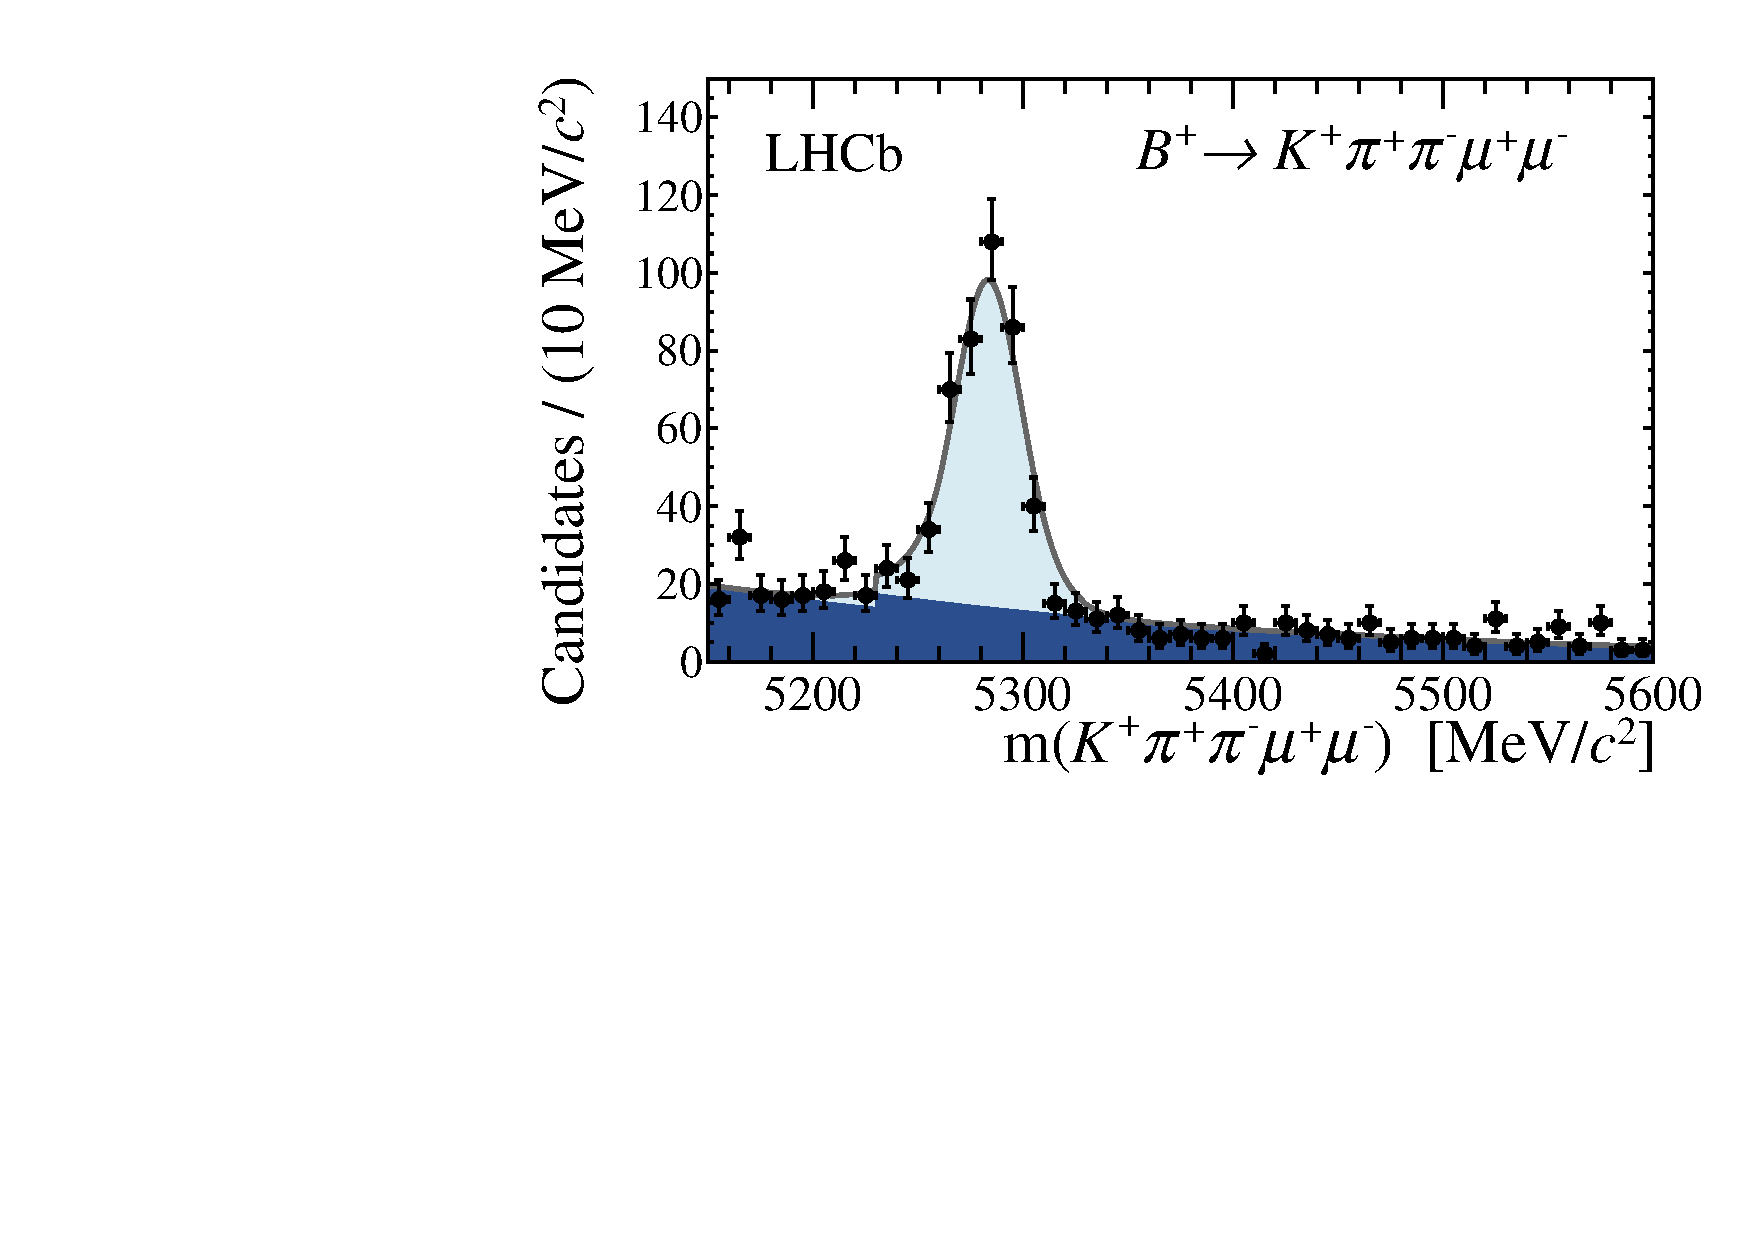
\includegraphics[width=0.48\textwidth]{b2kpipimumu}
    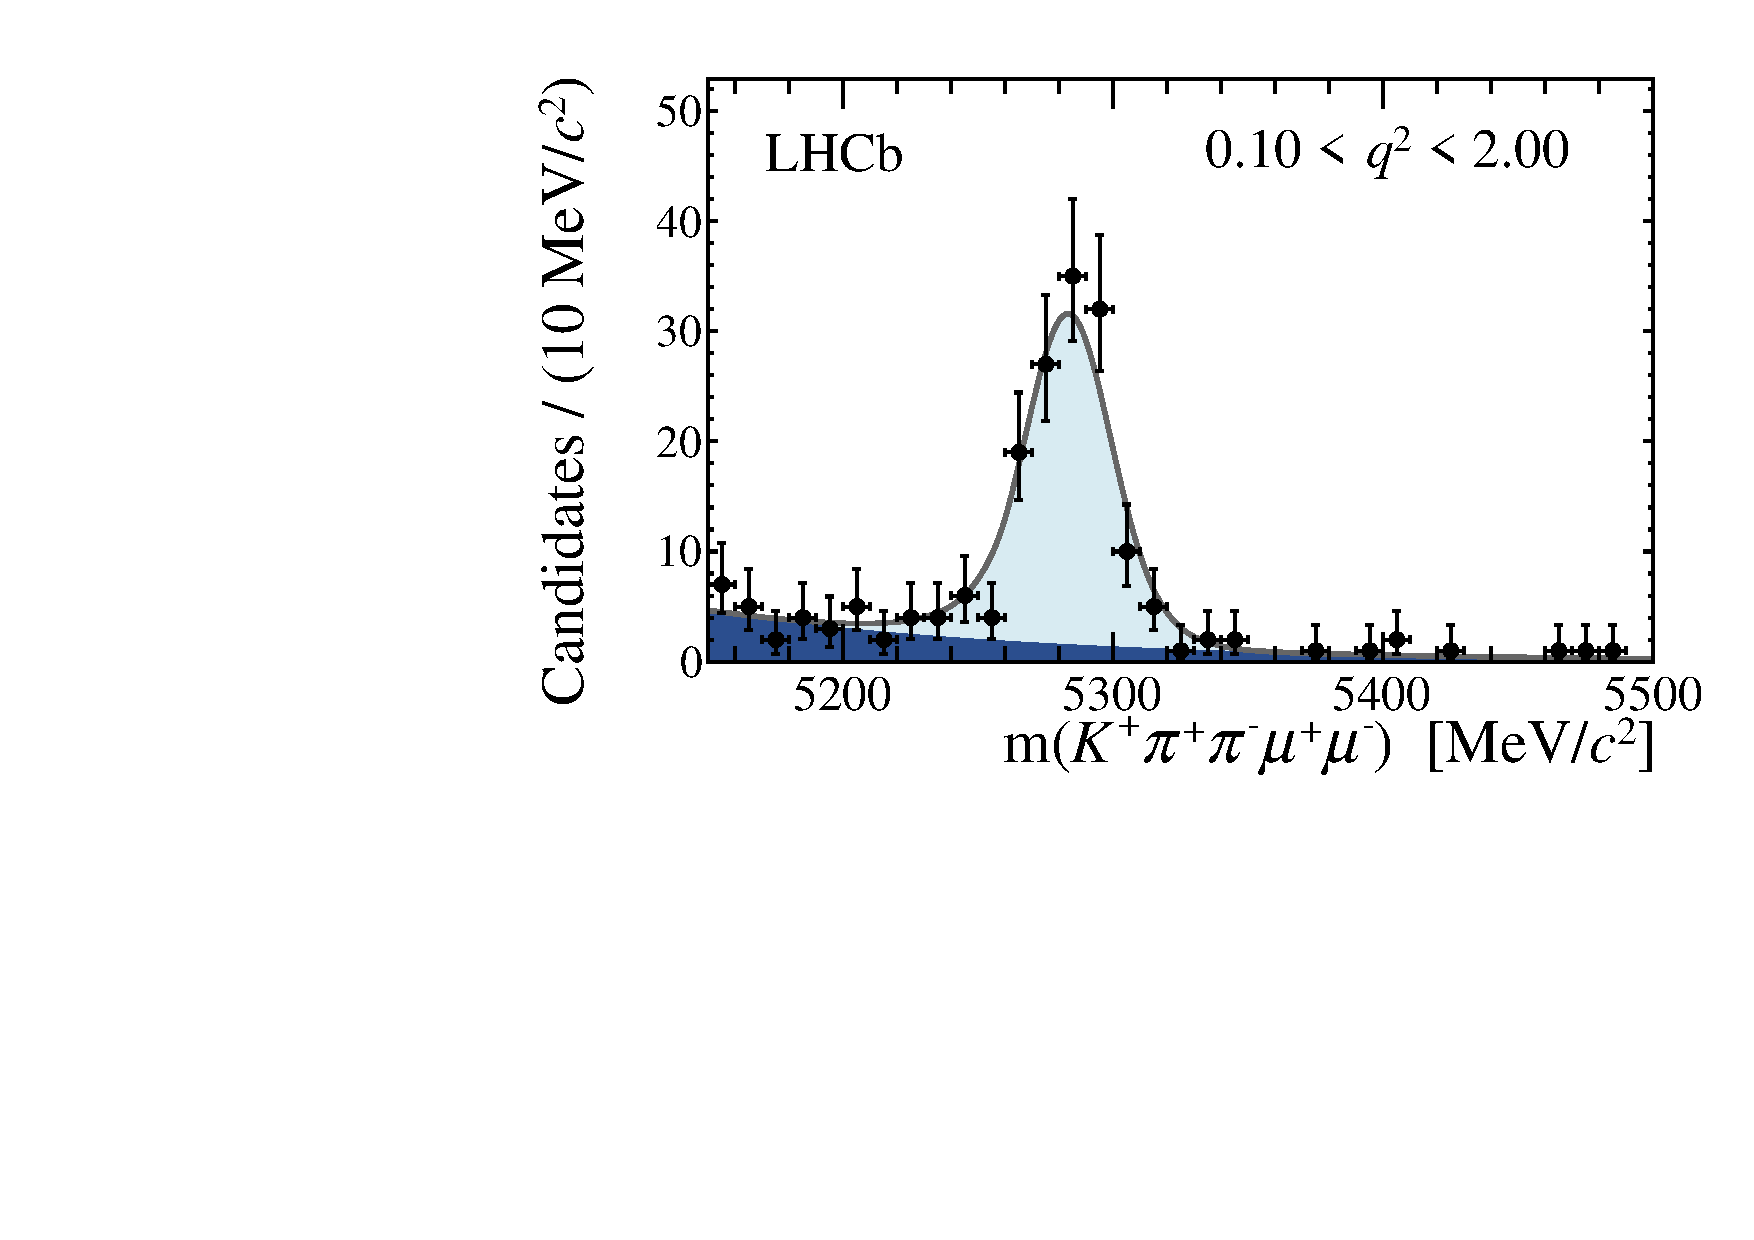
\includegraphics[width=0.48\textwidth]{kpipimumu_q2_r2}
    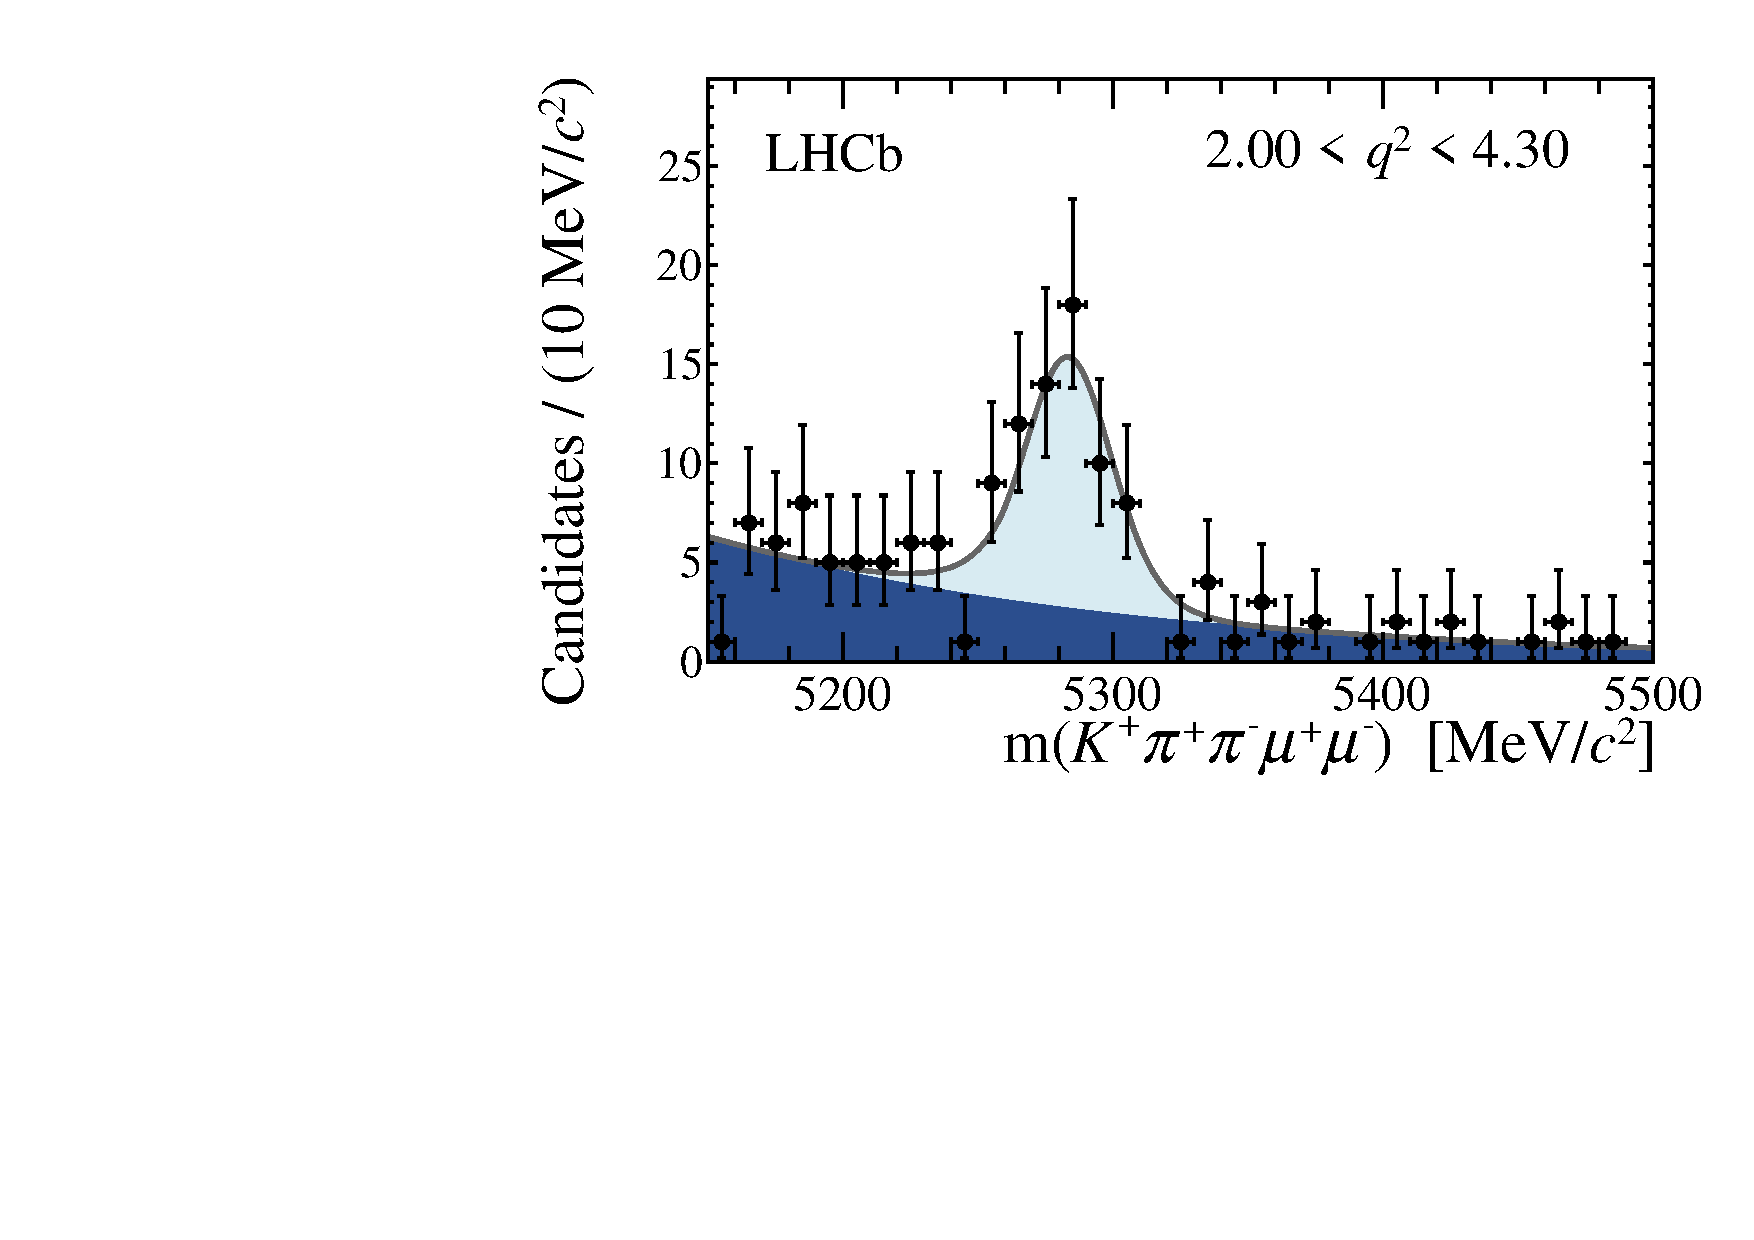
\includegraphics[width=0.48\textwidth]{kpipimumu_q2_r3}
    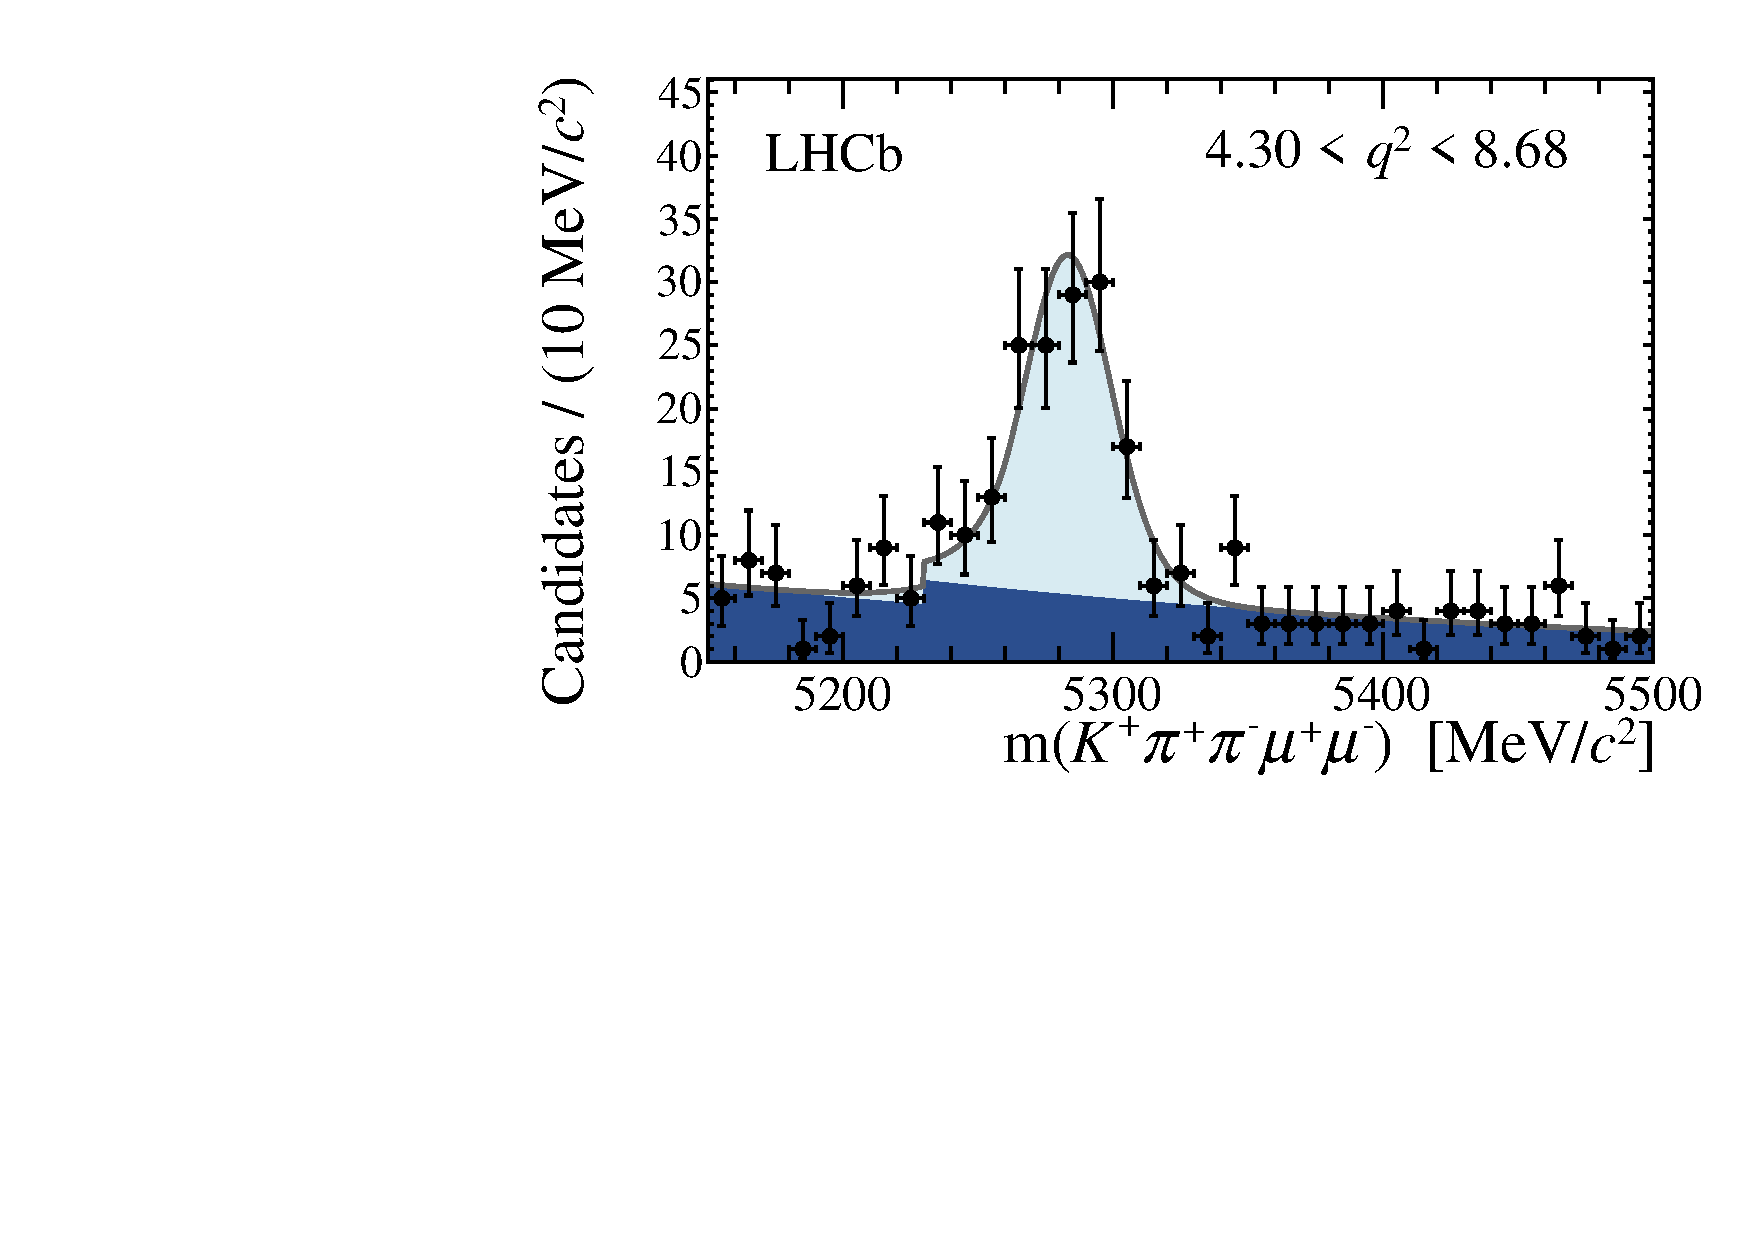
\includegraphics[width=0.48\textwidth]{kpipimumu_q2_r4}
    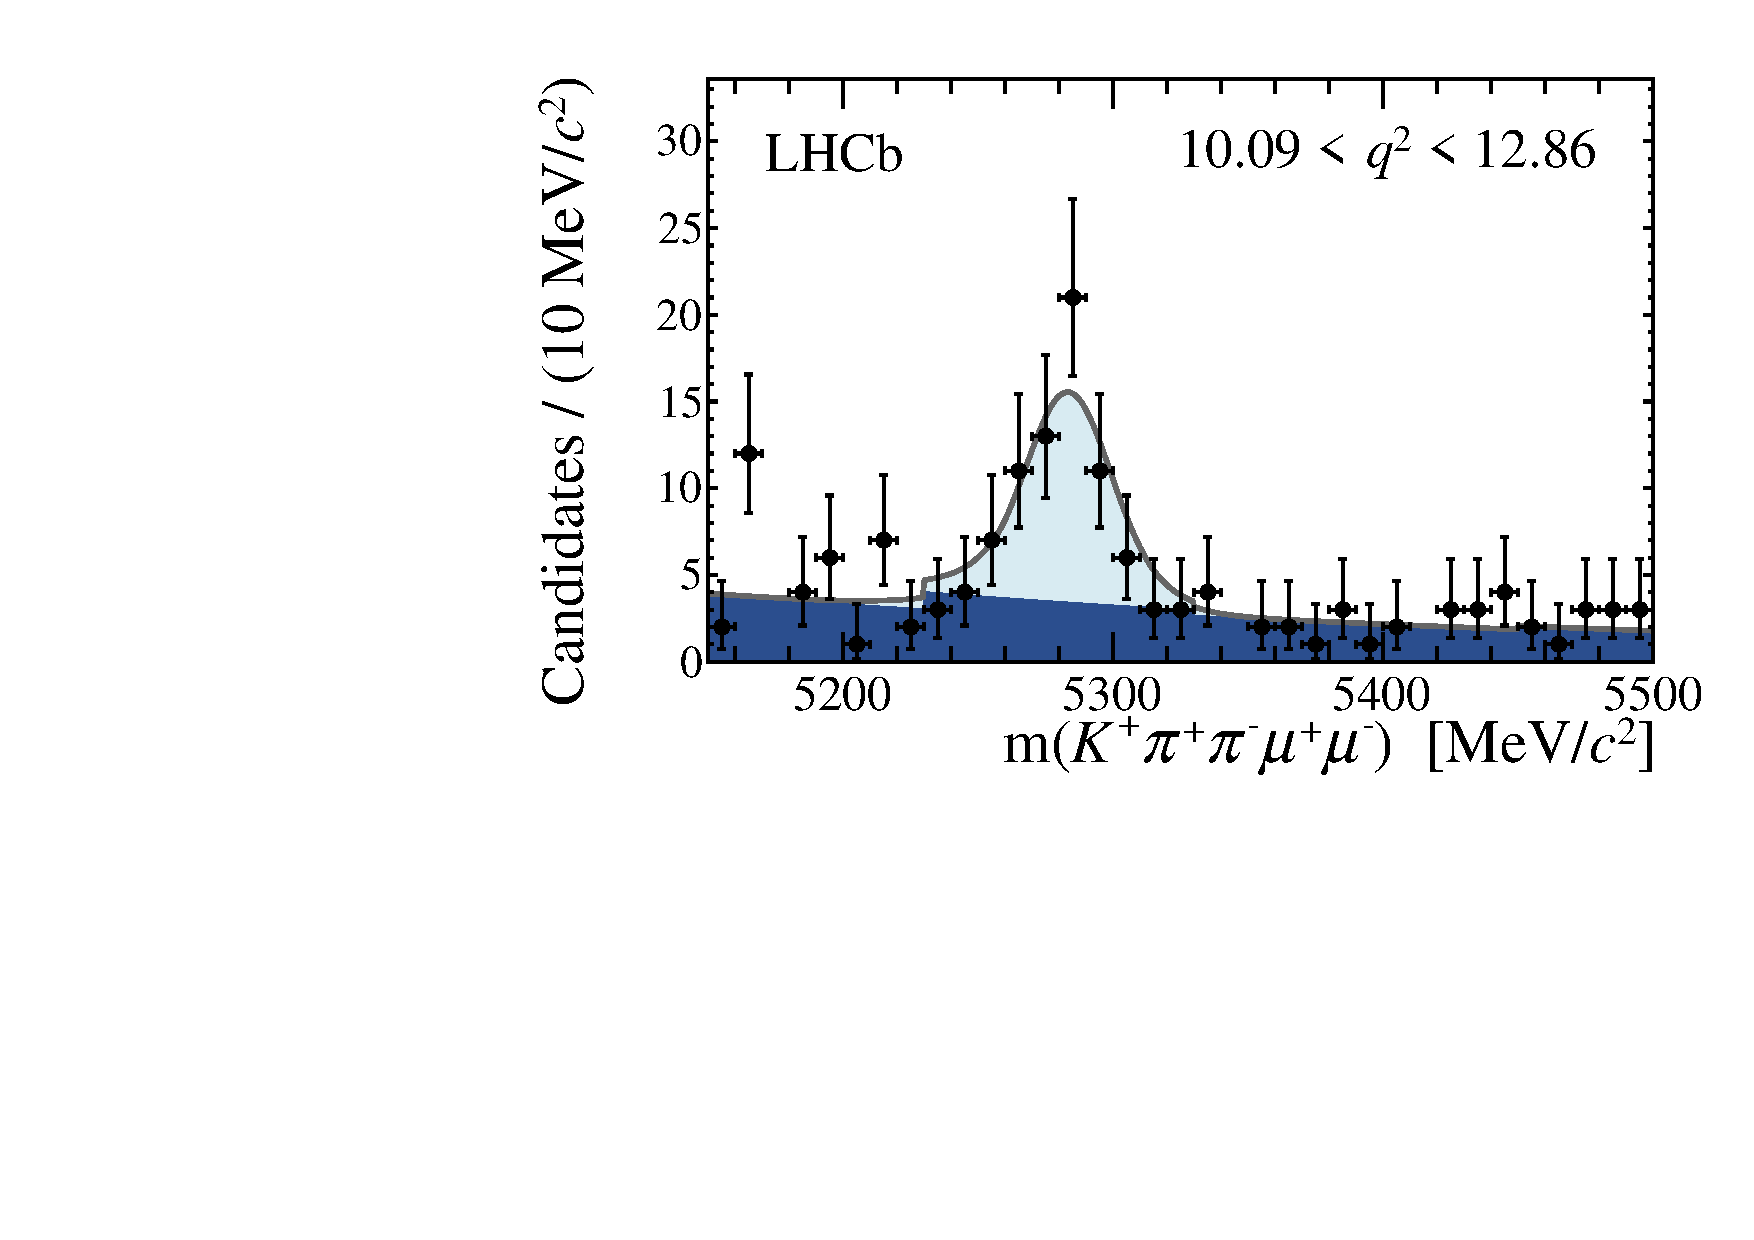
\includegraphics[width=0.48\textwidth]{kpipimumu_q2_r5}
    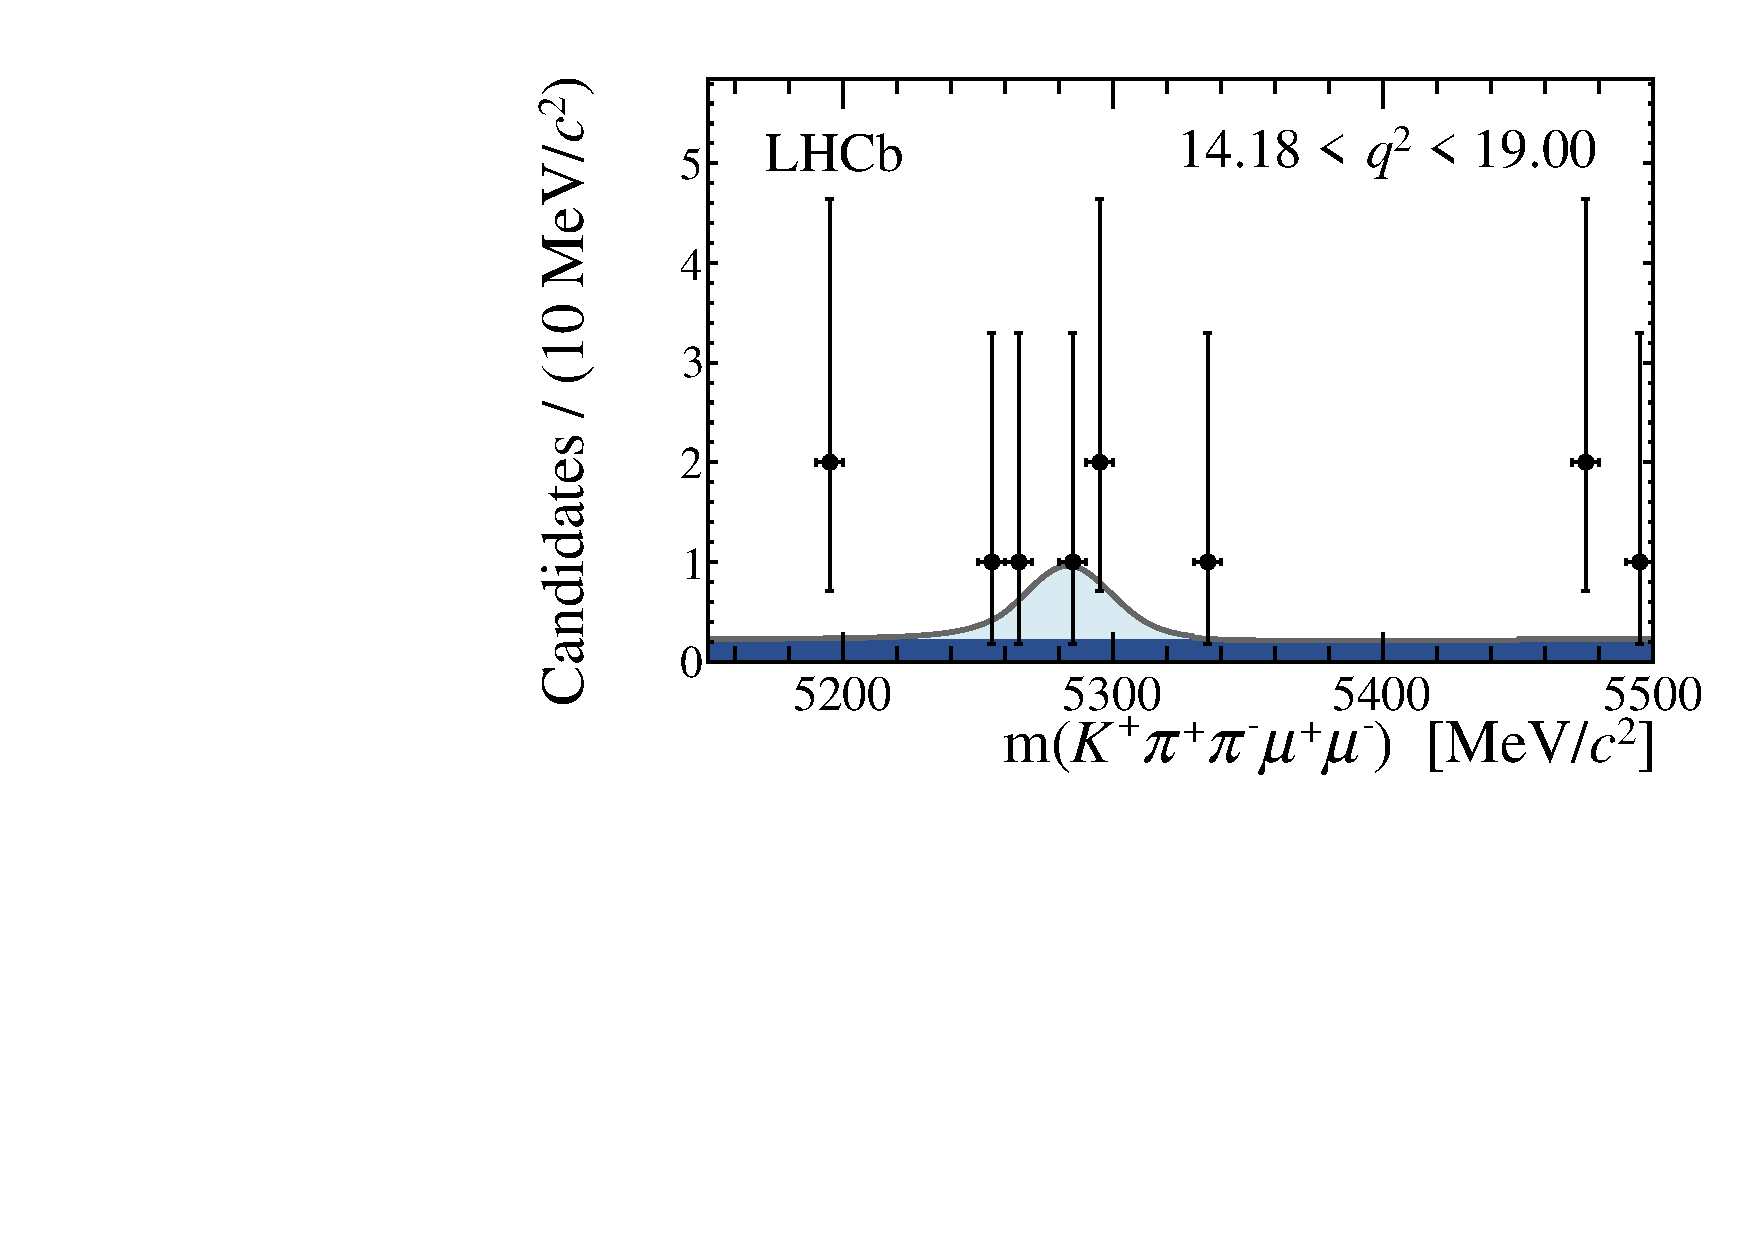
\includegraphics[width=0.48\textwidth]{kpipimumu_q2_r6}
    \caption[Fits to signal decay \btokpipimumu]
    {
      Invariant mass distributions of \btokpipimumu candidates in bins of \qsq with projections of
      fits overlaid, the upper left plot is a separate fit to the full \qsq range.
      The signal signal component (light blue) is modelled by the sum of two Gaussian
      distributions, and the background component (dark blue) is an exponential function.
      In the three \qsq bins $4.30<\qsq<8.68\gevgev$, $10.09<\qsq<12.86\gevgev$, and
      $14.18<\qsq<19.00\gevgev$ scaling factors in the background components are used to account
      the removal of the radiative tails of charmonium vetoes.
    }
    \label{fig:kpipi:q2fits}
  \end{center}
\end{figure}

%\begin{figure}[h]
  %\begin{center}
    %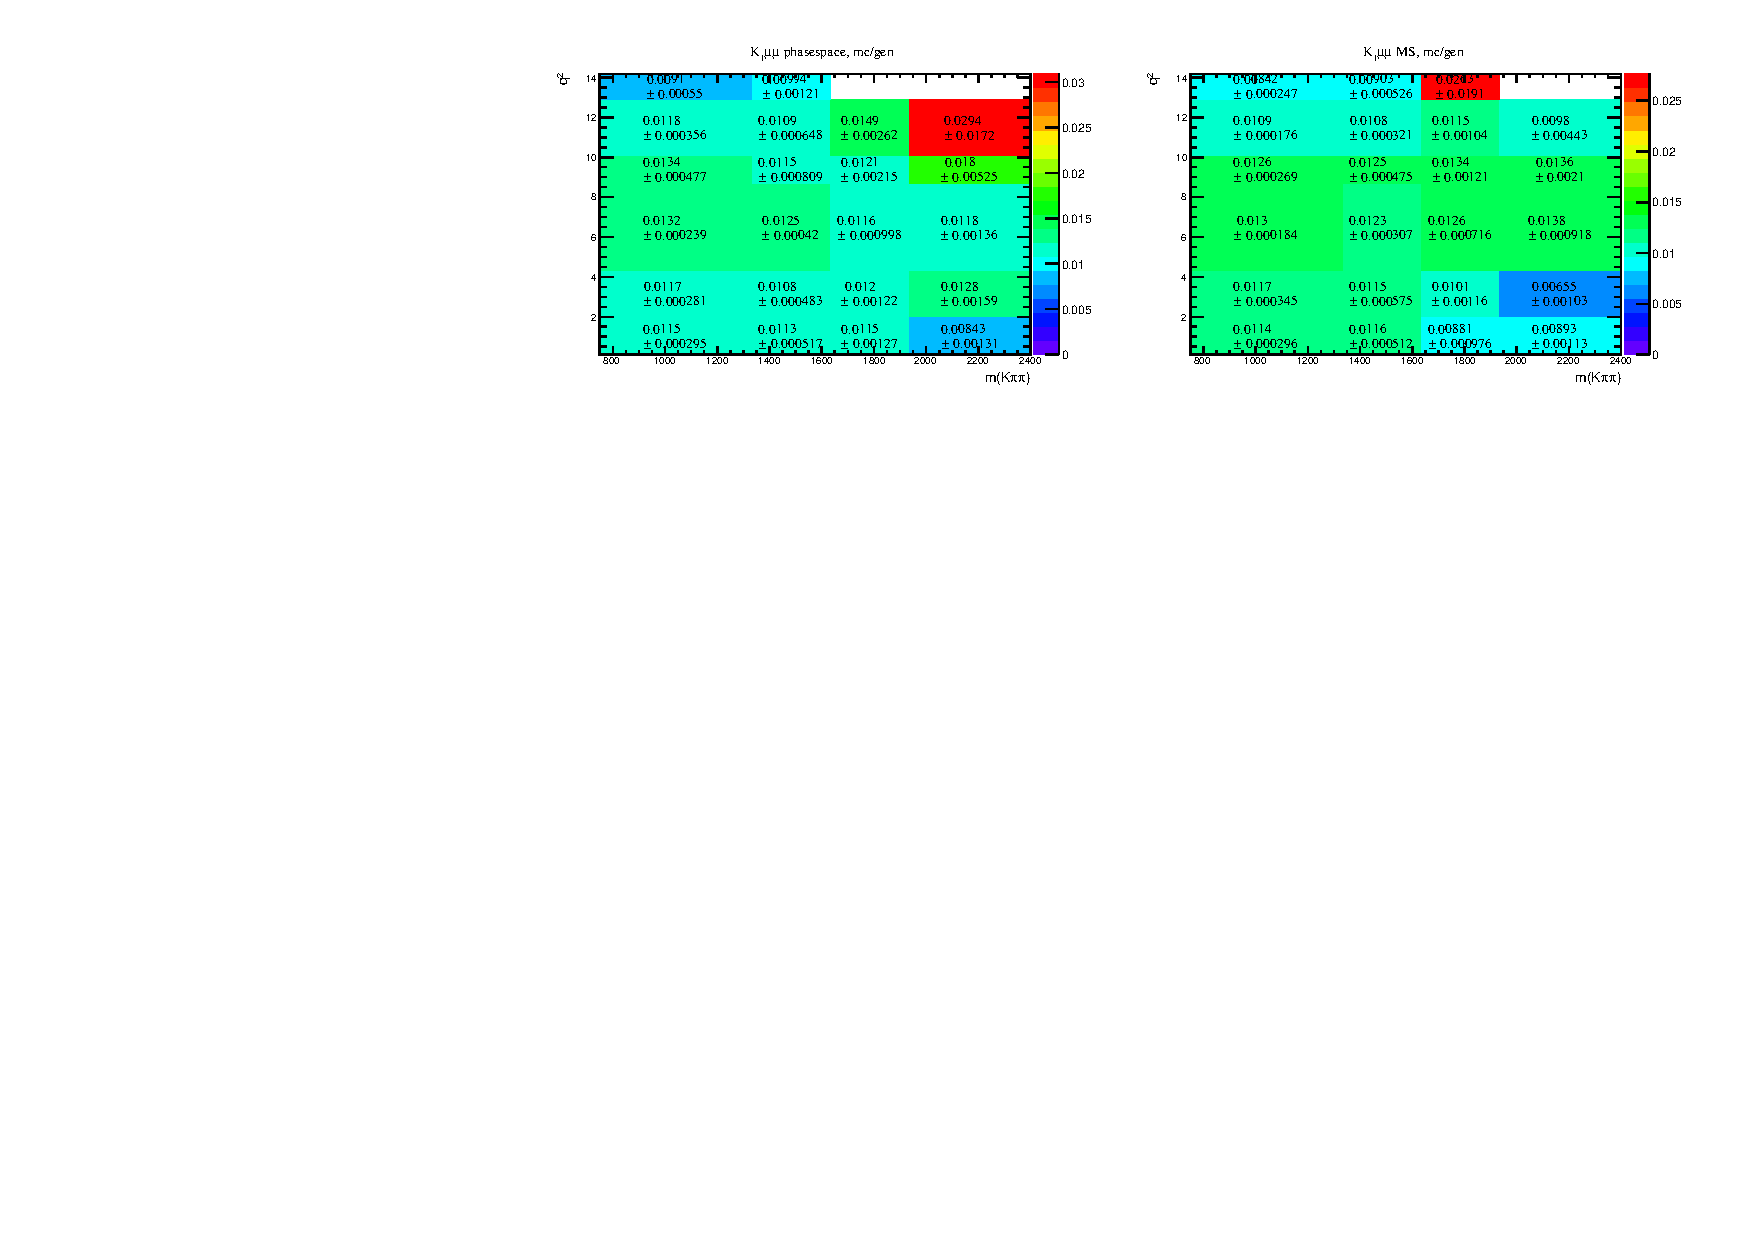
\includegraphics[width=0.48\textwidth]{q2vk1_eff}
    %\caption{ Efficiencies of reconstructed simulated events with respect to generator level
      %distributions of $\Bu\!\to K_1(1270)^+\mumu$ in bins of \qsq and \mass{\kpipi}.
      %The shape of the efficiency distribution is dominated by \qsq, and is relatively flat in
      %the \mass{\kpipi} dimension.
      %Vetoes \jpsi and \psitwos regions are indicated by black lines.
    %}
    %\label{fig:q2vk1eff}
  %\end{center}
%\end{figure}


Differential branching fractions were calculated according to \Eq{eq:kpipi:diffbf}, where yields
were extracted from fits in \Fig{fig:kpipi:q2fits}.
Results are shown graphically in \Fig{fig:kpipi:diffbf} and are given numerically --- along
with signal yields --- in \Tab{tab:kpipi:diffbf}.
These results also quote a number for the $1.0<\qsq<6.0\gevgev$ region, which is an area of lower
theoretical uncertainty for dimuon \fcnc decays, as it is away from the photon pole at low mass,
and away from the \jpsi at high mass.
Uncertainty from the normalization channel is fully correlated between all \qsq bins.
The sum over all \qsq bins results in an integrated branching fraction of
\begin{equation*}
  \BF\big( \btokpipimumu \big)=
  \big(3.43\,^{+0.23}_{-0.21}\stat\pm0.15\syst\pm0.14\normerr\big)\e{-7};
\end{equation*}
where quoted uncertainties are statistical, systematic and due to the errors on the branching
fraction of the normalization channel.
The fraction of signal events removed by the charmonium vetoes is determined from simulated
\decay{\Bp}{\kone{1270}\mumu} events % changing the form factors
to be $(21.3\pm1.5)\,\%$.
Finally, the adjusted integrated branching fraction is
\begin{equation*}
  \BF\big( \btokpipimumu \big)=
  \big(4.36\,^{+0.29}_{-0.27}\stat\pm0.21\syst\pm0.18\normerr\big)\e{-7}.
\end{equation*}
The statistical significance of this result is in excess of $20\stdev$ according to Wilks'
theorem~\cite{wilks1938}.

Since the uncertainty due to the normalization channel branching fraction is significant, the
ratio of branching fractions is also quoted
\begin{equation*}
  \frac{ \BF\big( \btokpipimumu \big) }{ \BF\big( \btopsitwosk \big) } =
  \big(6.95\,^{+0.46}_{-0.43}\stat\pm0.34\syst\big)\e{-4}.
\end{equation*}
%Where the value used is~\cite{PDG2012}
%$\BF_\mathrm{tot}\big(\btopsitwosk\big)$,
%and the uncertainty is fully correlated between \qsq bins.

{\renewcommand{\arraystretch}{1.2}
\begin{table}
  \begin{center}
    \caption[Differential branching fractions for the decay \btokpipimumu]
    {
      Signal yields and resulting differential branching fractions for the decay \btokpipimumu in
      bins of \qsq.
    }
    \label{tab:kpipi:diffbf}
    \begin{tabular}{ccc}\toprule
      \qsq bin $\left(\gevgev\right)$
      & $N_\sig$
      & $\tfrac{\dBF}{\dqsq}\;\left(\e{-8}\,\mathrm{GeV}^{-2}\right)$
      \\\midrule
      $[\pz0.10,\pz2.00]$ & $134.1\,^{+12.9}_{-12.3}$     & $7.01\,^{+0.69}_{-0.65} \pm 0.47$ \\
      $[\pz2.00,\pz4.30]$ & $\pz56.5\,^{+\pz9.7}_{-\pz9.1}$ & $2.34\,^{+0.41}_{-0.38} \pm 0.15$ \\
      $[\pz4.30,\pz8.68]$ & $119.9\,^{+14.6}_{-13.7}$     & $2.30\,^{+0.28}_{-0.26} \pm 0.20$ \\
      $[10.09,12.86]$     & $\pz54.0\,^{+10.1}_{-\pz9.4}$   & $1.83\,^{+0.34}_{-0.32} \pm 0.17$ \\
      $[14.18,19.00]$     & $\pzz3.3\,^{+\pz2.8}_{-\pz2.1}$ & $0.10\,^{+0.08}_{-0.06} \pm 0.01$ \\
      \littlerule
      $[\pz1.00,\pz6.00]$ & $144.8\,^{+14.9}_{-14.3}$     & $2.75\,^{+0.29}_{-0.28} \pm 0.16$ \\
      \bottomrule
    \end{tabular}
  \end{center}
\end{table}
}

\begin{figure}
  \begin{center}
    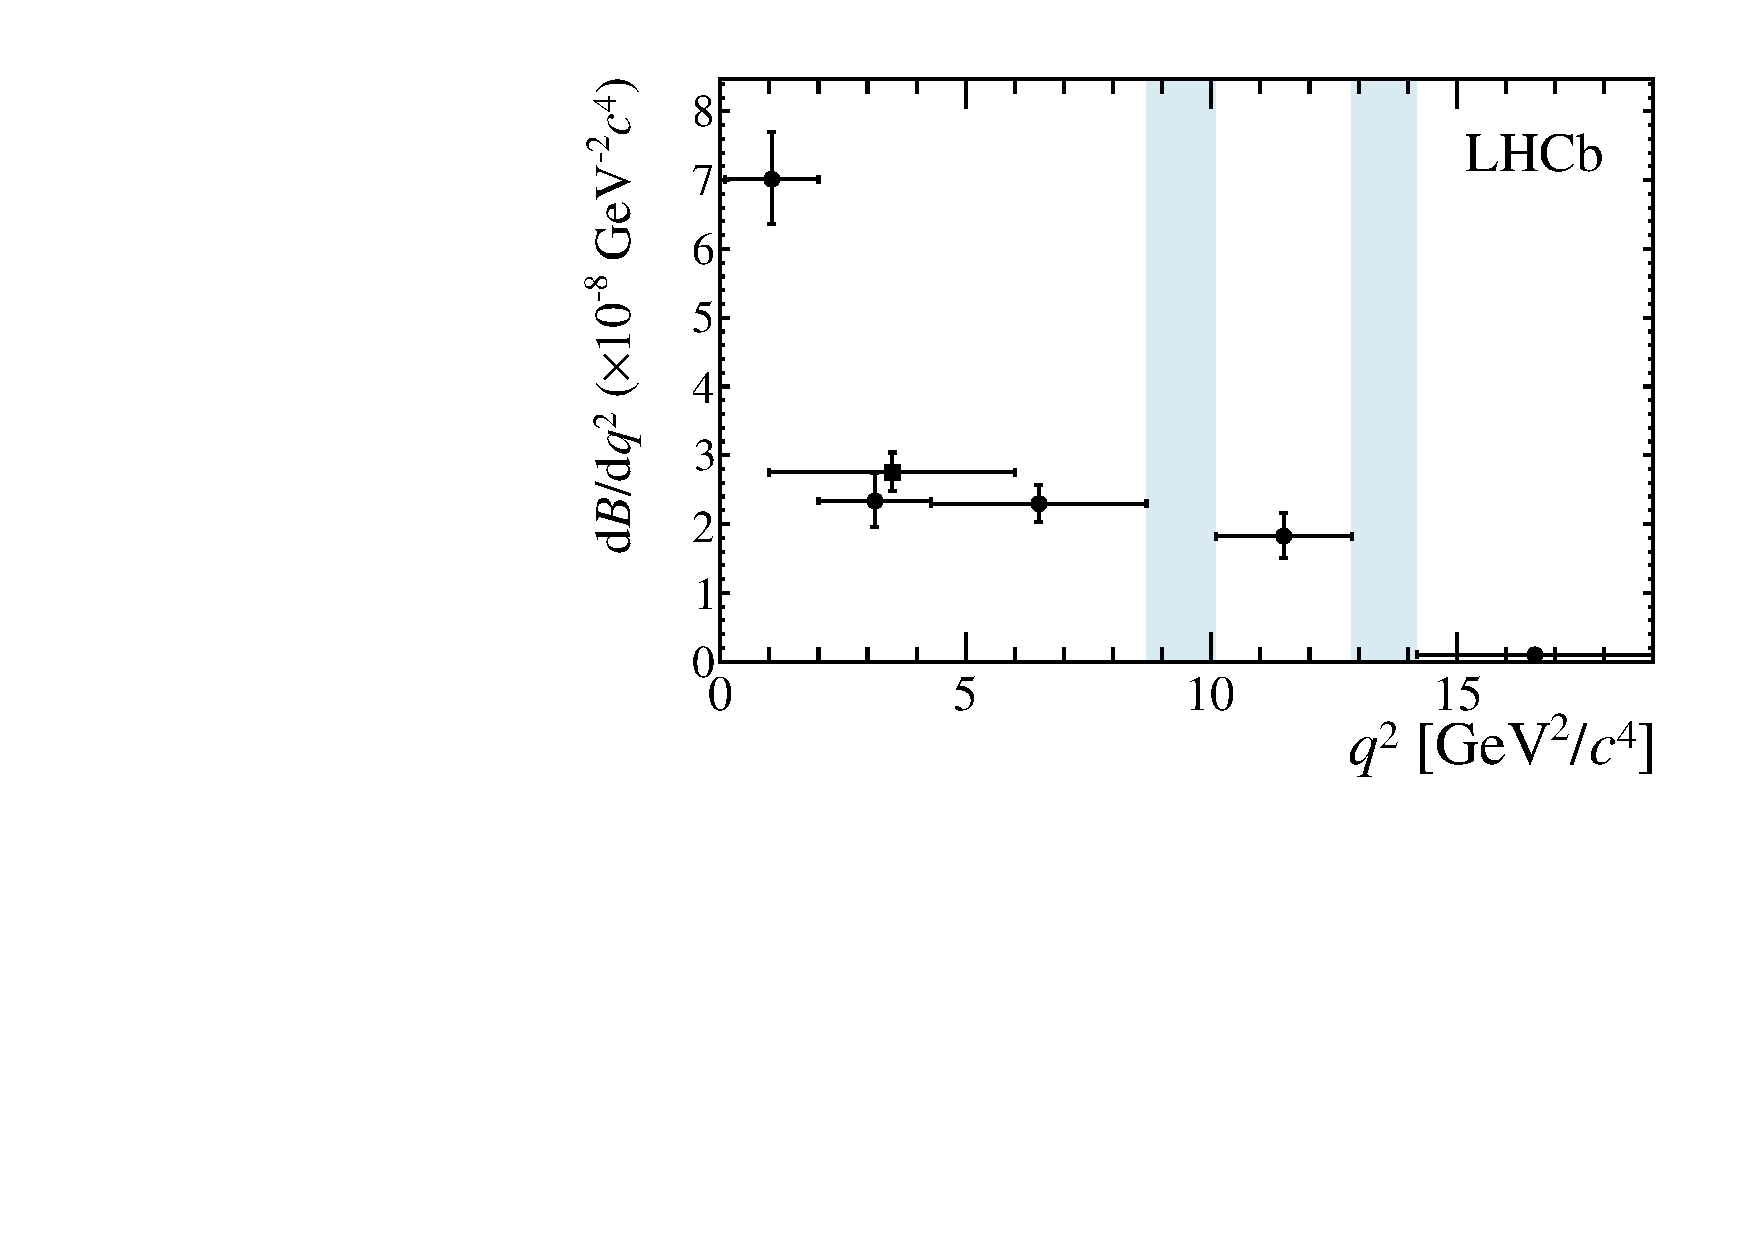
\includegraphics[width=0.6\textwidth]{diffbf_16}
    \caption[Differential branching fractions of \btokpipimumu]
    {
      Differential branching fraction $\tfrac{d}{\dqsq}\BF\left(\btokpipimumu\right)$
      as given in Table~\protect\ref{tab:kpipi:diffbf}, where the
      errors shown include both statistical and systematic uncertainties.
      Shaded areas indicate the vetoed \jpsi and \psitwos resonances.
      The result for the $1.0<\qsq<6.0\gevgev$ region which has reduced theoretical uncertainties
      is also shown.
    }
    \label{fig:kpipi:diffbf}
  \end{center}
\end{figure}

Figure~\ref{fig:kpipi:kpipi} shows the background subtracted invariant mass distribution's of the
\kpipi system in the case of both decays \btojpsikpipi and \btokpipimumu.
Numerous broad resonances are visible in the distributions.
The \kpipi system from the resonant \btojpsikpipi decay shows significant, though not dominant,
contributions from the \kone{1270} state.
There is also a contribution visible as $m_\kpipi\simeq1750\mev$, similar to resonances seen by
\belle~\cite{Guler:2010if}.
However, there are significant differences between the invariant mass distributions of the \kpipi
system in the decays \btojpsikpipi and \btokpipimumu.
These differences can be explained by differeces in the allowed spin states due to the pseudoscalar
\jpsi.


\begin{figure}
  \begin{center}
    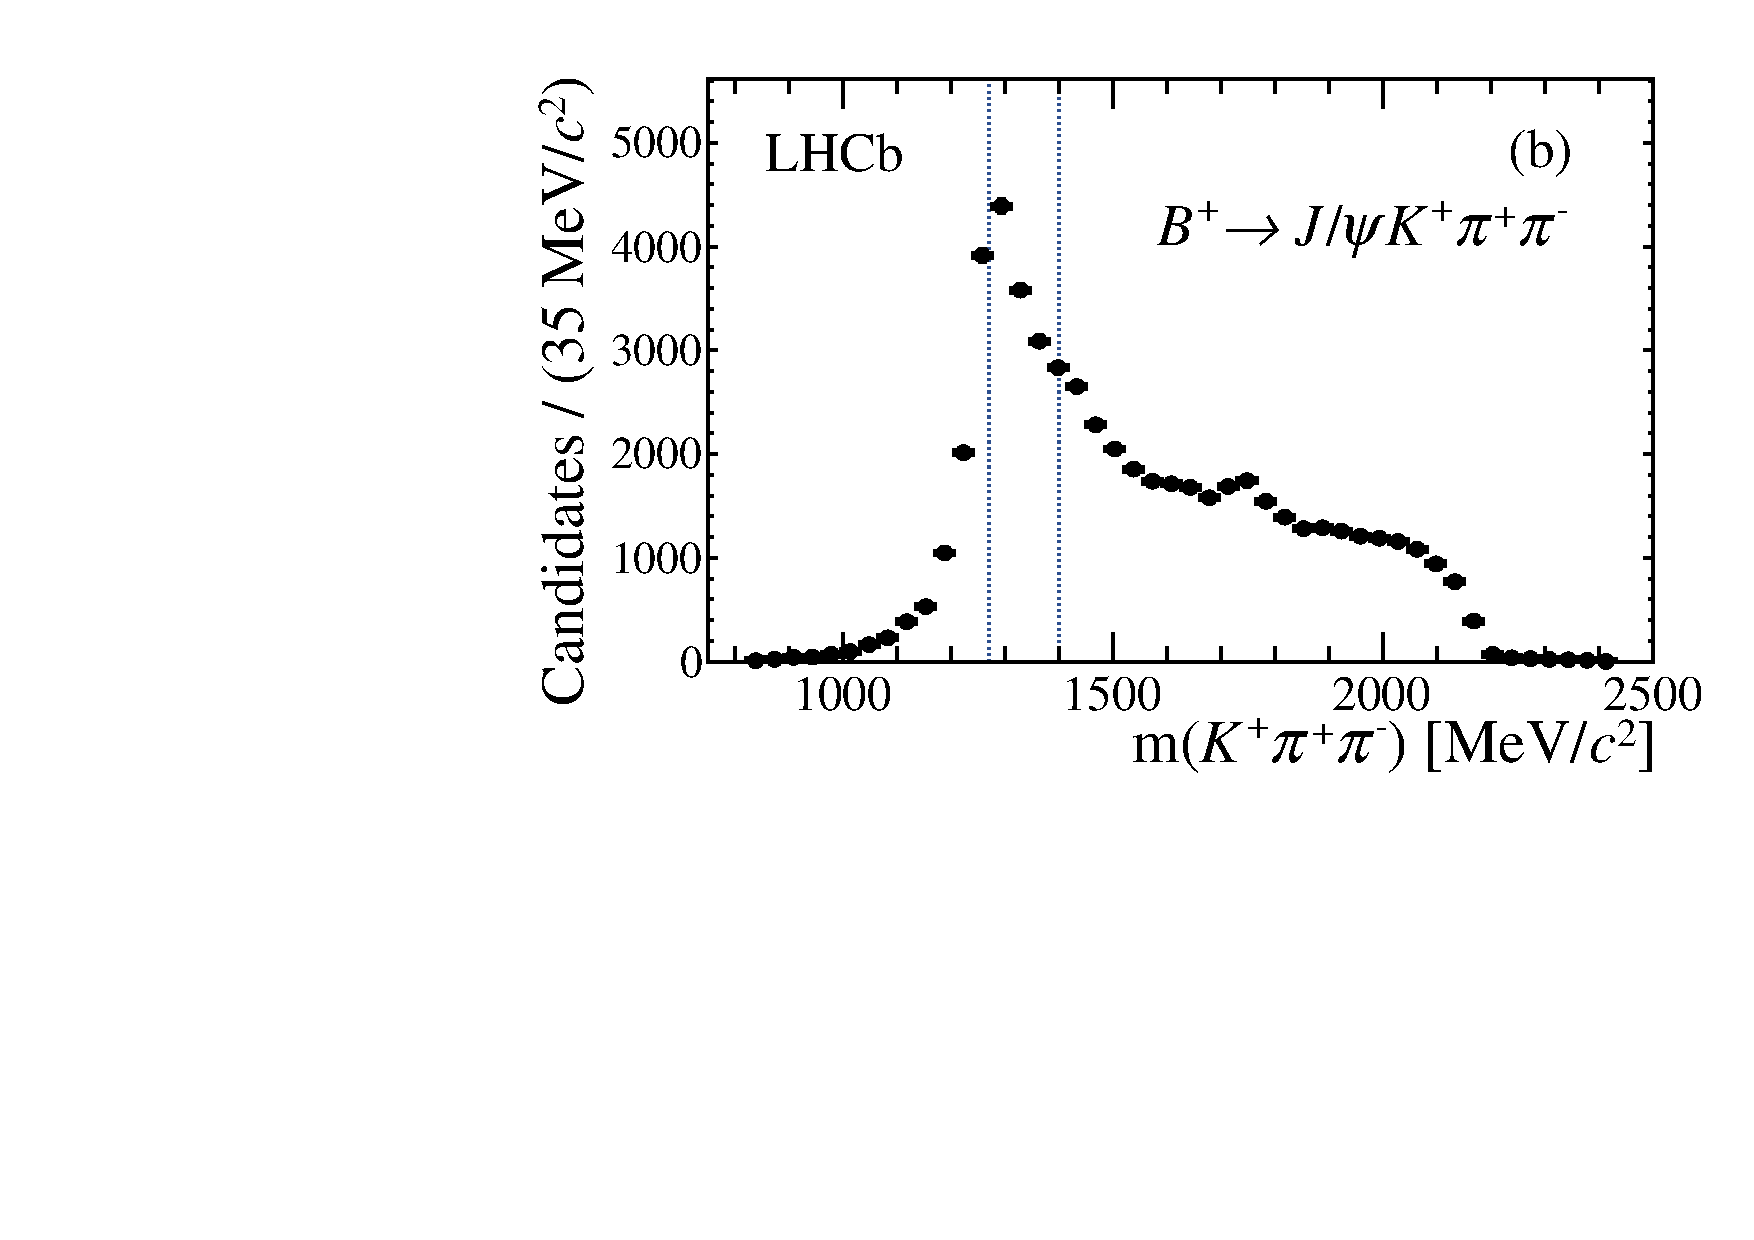
\includegraphics[width=0.48\textwidth]{kpipi_fromjpsi}
    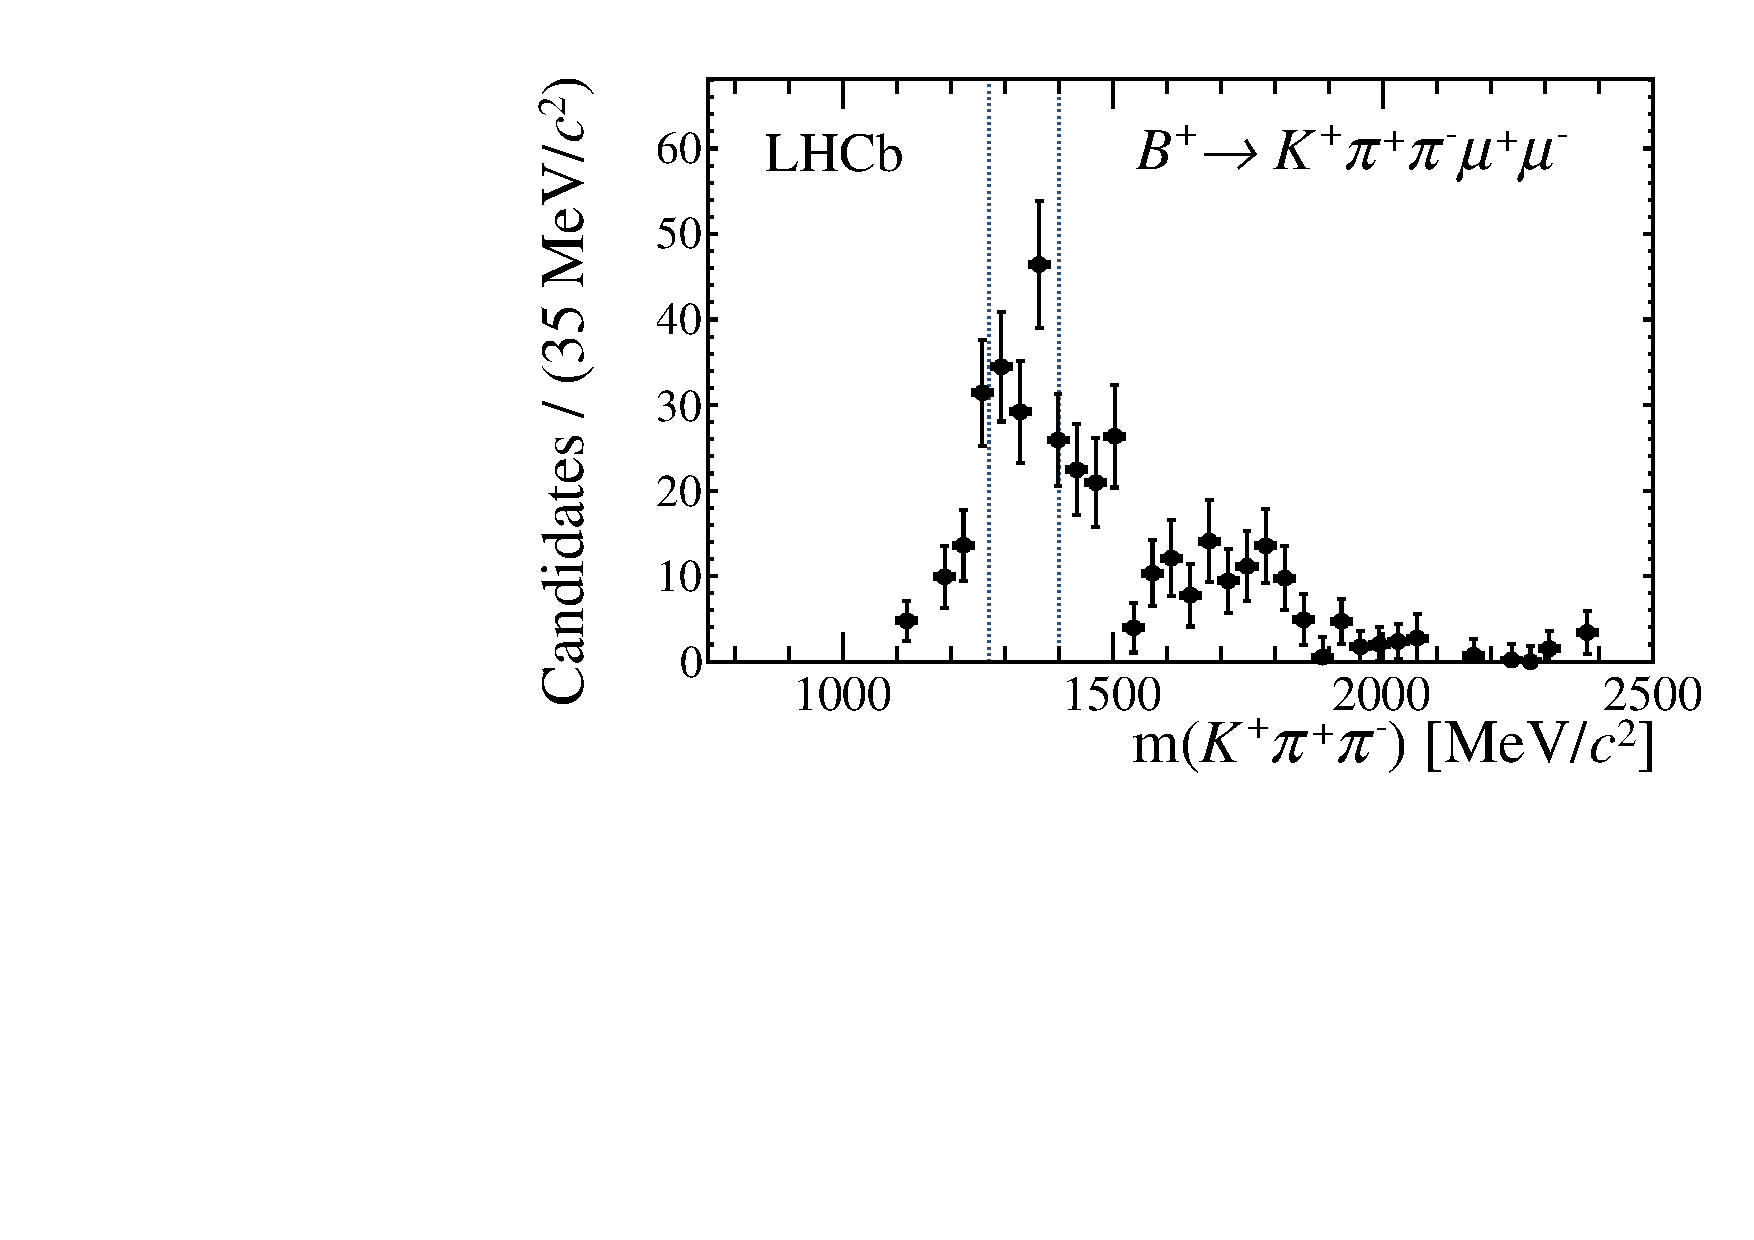
\includegraphics[width=0.48\textwidth]{kpipi_frommumu}
    \caption[Invariant mass distributions of \kpipi in data]
    {
      Invariant mass distributions of the \kpipi system, from the
      (left) control channel \btojpsikpipi, and the
      (right) signal decay \btokpipimumu
      which have been background subtracted
      using the \emph{sPlot}~\cite{splot} technique.
      The vertical lines indicate the central masses of the \kone{1270} and \kone{1400}
      resonances.
    }
    \label{fig:kpipi:kpipi}
  \end{center}
\end{figure}



\subsection{Systematic uncertainties}
\label{ssec:kpipi:syst}

Systematic uncertainties introduced to the measurement of the differential branching fraction of
\btokpipimumu can be categorised into three main categories:
corrections applied to simulated events for the efficiency calculation;
models used to describe the signal and normalization channel shapes; and
modelling of the signal decay.

% Reweighting and PID
Section~\ref{sec:hhh:eff} describes the process of correcting simulated events such that they best
describe data.
This procedure introduces systematic uncertainties which must be accounted for.
This is done by recalculating the relative efficiency for each \qsq bin:
without reweighting track multiplicity and the \chisq of the fit to the \Bp vertex;
without accounting for differences in tracking and {\tt isMuon} efficiencies;
and without performing PID resampling.
The resulting systematic uncertainty from the selection was assigned a value of $1\pc$.
Each source of uncertainty is treated separately, and the total systematic uncertainty is taken to
be the difference in the branching fraction with the newly calculated relative efficiency.
%{selection 1\%}
%{trigger 1\%}

% Fits
In order to assess the degree of uncertainty introduced by the distributions used to model the
signal and background components.
The systematic uncertainty is taken to be the difference between the nominal branching fraction,
and the branching fraction recalculated using different signal or background components in the fit.
A single Gaussian with a power-law tail is used as an alternative signal model and --- in a
different fit --- a linear function is used to describe the background.
The modelling of the mass distributions led to a systematic uncertainty of $2\pc$.

The way the signal decay is modelled in simulation were the source of numerous systematic
uncertainties.
Efficiencies were calculated using simulated data using the model described in
\Ref{Hatanaka:2008gu}, but this is imperfect for a number of reasons.
This model does not match data in \qsq or $m_\kpipi$; it also assumes that $\thetakone=-34^\circ$,
and was used to determine the fraction of signal removed by charmonium vetoes.

To assess the systematic introduced by the difference between the \qsq distribution in data and
simulation a different decay model was used.
Rather than the efficiency for the signal channel being determined from simulated
\decay{\Bp}{\kone{1270}\mumu} generated with the model in \Ref{Hatanaka:2008gu}, it was decayed
using a phasespace model.
The differences in the invariant mass distribution of \kpipi cannot be assessed using simulation
because of the difficulties associated with theoretically describing \kpipi resonances.
Instead, the signal efficiencies are calculated after being reweighted to match the sWeighted
$m(\kpipi)$ distribution from signal, as shown in \Fig{fig:kpipi:kpipi}.
%Systematic uncertainties from these two sources are assessed by redetermining branching fractions
%using these new signal efficiencies.

The value of the mixing angle \thetakone has been a source of some theoretical contention, where
$\thetakone=-34^\circ$ or
$-57^\circ$~\cite{PhysRevD.47.1252,Tayduganov:2011ui,Hatanaka:2008xj,Cheng:2011pb,Divotgey:2013jba,Cheng:2013cwa}.
But, more recently measurements favour a value of approximately
$-(34\pm13)^\circ$~\cite{Hatanaka:2008xj,Cheng:2011pb,Divotgey:2013jba,Cheng:2013cwa}.
To estimate the systematic uncertainty associated with this value, the simulated data was
reweighted on an event-by-event basis such that the value of \thetakone was varied by $1\,\sigma$.
%This was done by interfacing with \evtgen~\cite{Lange:2001uf} directly.

%The probability of a particle decaying into a given final state is done in \evtgen using
%a probability density function --- based on the decay model --- which is
%dependent upon the momenta of the final state particles.
%By calculating the probability of the decay with $\thetakone=-34^\circ$, and other angles, one can
%reweight the simulated data to match data from any angles.

The signal efficiency was recalculated after varying the \thetakone by $1\,\sigma$ in simulated
\decay{\Bp}{\kone{1270}\mumu} events.
Branching fractions were then evaluated using these new efficiencies, and the maximum difference
from the nominally calculated value is taken as the systematic uncertainty.
The same procedure was used to calculate systematics with respect to $\thetakone=-57^\circ$, and
the values are found to be consistent with the theoretically favoured value of $-(34\pm13)^\circ$;
leading to an assigned uncertainty of \approx$1.5\pc$.

Charmonium vetoes removes a percentage of signal candidates, that must be accounted for in order to
calculate the total integrated branching fraction.
This fraction is subject to a systematic uncertainty due to the mismodelling of the \qsq
distribution in the simulated signal events.
Form factors in \Ref{Hatanaka:2008gu} gave the central value of $21.3\,\%$.
Varying these form factors at generator level by a random number forms a Gaussian distribution,
whose standard deviation is the uncertainty on the form factor.
This is done multiple times and leads to an uncertainty of $1.5\,\%$.


%The trigger selection also introduces some systematic uncertainty...
%TISTOS method
%$$
 %e_TOS = N_tis\&tos / N_tis
%$$
%tis is number of events triggered independently of the signal candidate
%tis\&tos is number of evennts triggered by both
%small disagreements at L0, use ratio of L0 for data and simulation to rw MC redetermined relative
%effs


%\subsubsection{Selection}
%\subsubsection{Trigger}

%\subsubsection{Peaking backgrounds}
%Negligible
%\subsubsection{Relative uncertanty}
%Negligible





\begin{table}
  \caption[Systematic uncertainties on the differential branching fraction of \btokpipimumu]
  {
    Systematic uncertainties on the differential branching fraction of
    %\mbox{${\rm d}{\cal B}(\Bu\to\Kp\pip\pim\mup\mun)/{\rm d}q^2$}
    \btokpipimumu in bins of $q^2$ $[\times 10^{-8} \gev^{-2}]$.
  }
  \label{tab:kpipi:syst}
  \begin{center}
  \begin{tabular}{lccccc}\toprule
    & \multicolumn{5}{c}{$q^2$ bin $[\gev^2]$}\\
    Source
    & \celll{$[0.10,$}
    & \celll{$[2.00,$}
    & \celll{$[4.30,$}
    & \celll{$[10.09,$}
    & \celll{$[14.19,$}
    %& $[\pz2.00,\pz4.30]$
    %& $[\pz4.30,\pz8.68]$
    %& $[10.09,12.86]$
    %& $[14.19,19.0]$
    \\
    & \celll{$\phantom{[}2.00]$}
    & \celll{$\phantom{[}4.30]$}
    & \celll{$\phantom{[}8.68]$}
    & \celll{$\phantom{[}12.86]$}
    & \celll{$\phantom{[}19.00]$}
    %& $[\pz2.00,\pz4.30]$
    %& $[\pz4.30,\pz8.68]$
    %& $[10.09,12.86]$
    %& $[14.19,19.0]$
    \\ \midrule
    $\BF\big(\btopsitwosk\big)$      &   0.288 &   0.096 &   0.094 &   0.075 &   0.004 \\  % x10e-8
    %Tracking efficiency    &   0.080 &   0.020 &   0.024 &   0.012 &   0.000 \\  % x10e-8
    %Reweighting            &   0.106 &   0.006 &   0.034 &   0.006 &   0.000 \\  % x10e-8
    %PID efficiency         &   0.060 &   0.057 &   0.041 &   0.044 &   0.002 \\  % x10e-8
    %Muon PID efficiencies  &   0.055 &   0.020 &   0.018 &   0.010 &   0.000 \\  % x10e-8
    %Signal mass model      &   0.138 &   0.052 &   0.052 &   0.039 &   0.002 \\  % x10e-8
    %Background mass model  &   0.154 &   0.038 &   0.052 &   0.093 &   0.003 \\  % x10e-8
    %\qsq model             &   0.087 &   0.047 &   0.027 &   0.094 &   0.002 \\  % x10e-8
    %$K^+\pipi$ composition &   0.175 &   0.009 &   0.010 &   0.061 &   0.004 \\  % x10e-8
    %\thetakone             &   0.110 &   0.036 &   0.062 &   0.003 &   0.001 \\  % x10e-8
    %Relative efficiencies  &   0.014 &   0.005 &   0.003 &   0.003 &   0.000 \\  % x10e-8
    %Peaking backgrounds    &   0.000 &   0.000 &   0.126 &   0.000 &   0.000 \\  % x10e-8
    %Trigger                &   0.152 &   0.052 &   0.042 &   0.011 &   0.000 \\  % x10e-8
    %\littlerule
    Corrections to simulation & 0.218 & 0.082 & 0.074 & 0.048 & 0.002 \\
    \kpipi composition        & 0.175 & 0.009 & 0.010 & 0.061 & 0.004 \\
    Value of \thetakone       & 0.110 & 0.036 & 0.062 & 0.003 & 0.001 \\
    Modelling \qsq            & 0.087 & 0.047 & 0.027 & 0.094 & 0.002 \\
    Mass model: background    & 0.154 & 0.038 & 0.052 & 0.093 & 0.003 \\
    Mass model: signal        & 0.138 & 0.052 & 0.052 & 0.039 & 0.002 \\
    Relative efficiencies     & 0.014 & 0.005 & 0.003 & 0.003 & 0.000 \\
    Peaking backgrounds       & 0.000 & 0.000 & 0.126 & 0.000 & 0.000 \\
    \littlerule
    Total    & 0.473 & 0.154 & 0.201 & 0.175 & 0.007 \\
    \bottomrule
    \end{tabular}
  \end{center}
\end{table}
%\scalebox{0.8}{
  %{\setlength{\tabcolsep}{0.25em}









